We use an MPC controller with a quadratic and a linear cost for comparison.
The finite RHC approach involves optimizing a cost function subject to the dynamics of the system and the constraints, over a finite horizon of time \cite{Mayne2000}. After an optimal sequence of control inputs are computed, the first input is applied, then at the next step the optimization is solved again.

%\begin{figure}
%\centering
%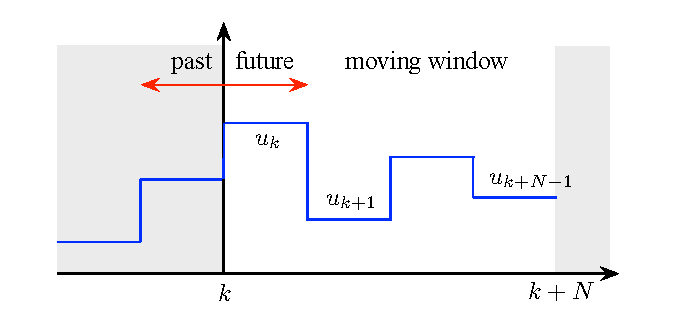
\includegraphics[scale=0.8]{figures/mpc_horizon.eps}
%\caption{Finite-horizon moving window of MPC: at time $k$, the MPC optimization problem is solved for a finite length window of $N$ steps and the first control input $u_k$ is applied; the window then recedes one step forward and the process is repeated at time $k+1$.}
%\captionsetup{justification=centering}
%\label{F:mpc}
%\end{figure}

The objective of the controller is to minimize the energy usage $c^Tu$ while maintaining a desired level of thermal comfort $x_{ref}$.
Therefore, at time step $k$, we solve a continuously linearized MPC problem to determine the optimal sequence of inputs $[u_{\mathrm{k|k}},\dots,u_{\mathrm{k+N-1|k}}]$:
\begin{subequations}
\begin{align}
\text{min } & \sum_{j=1}^{N} ({x}^T_{\mathrm{k+j|k}} - x_{ref}) \mathcal{Q} ({x}_{\mathrm{k+j|k}} - x_{ref}) + c^Tu_{\mathrm{k+j-1}} +  \lambda\epsilon_j\\
\text{s.~t. } & \ \ x_{\mathrm{k+j|k}} =  Ax_{\mathrm{k|k}} + B u_{\mathrm{k+j-1|k}} + B_d d_{\mathrm{k+j-1|k}} \label{SE:mpc1} \\
& \ \ \ \ \ B = B_u + B_{xu}[x_{\mathrm{k|k}}] + B_{du}[d_{\mathrm{k+j-1|k}}] \label{SE:mpc2}\\
& \ \ \ \ \ \ \ \ \ \ \ \ \ \ \ \underline{u} \leq u_{\mathrm{k+j-1|k}} \leq \bar{u}\\ 
& \ \ \ \ \ \ \ \ \ \ \ \ \underline{x}-\epsilon_j \leq x_{\mathrm{k+j|k}} \leq \bar{x} + \epsilon_j\\\
& \ \ \ \ \ \ \ \ \ \ \ \ \ \ \epsilon_j \geq 0, \ j = 1,\dots,N,
\end{align}\label{E:mpc}
\end{subequations} 
\noindent where $\mathcal{Q} \in \R^{12 \times 12}$ has all zeros except at $\mathcal{Q}^{(1,1)}$ corresponding to the zone temperature, $c \in \R^{4}$ is proportional to cost of using each actuator and $\lambda$ penalizes the slack variables.